\documentclass[sigconf]{acmart} %Recommended doc class from Lins;
\acmConference[Robo-Maze Blast Project]{
	University for Applied Sciences Hamburg\\
	Department of Computer Science}{2025}{Hamburg, Germany}
% Remove conference-specific formatting
\settopmatter{printacmref=false}  % Disables "ACM Reference Format"
\setcopyright{none}               % Removes copyright notice

\acmBooktitle{}                   % Removes booktitle
\acmDOI{}                         % Removes DOI
\renewcommand{\acmPrice}{}        % Removes price
% Language setting
% Replace `english' with e.g. `spanish' to change the document language
\usepackage[english]{babel}
\usepackage[ruled,vlined]{algorithm2e}
% Set page size and margins
% Replace `letterpaper' with `a4paper' for UK/EU standard size

% Useful packages
\usepackage{amsmath}
\usepackage{graphicx}
\usepackage{alltt}

\title{Robo-maze Blast Report}
\author{Dogà Sara}
\author{Widmann Lukas}
\author{Askar Sami}

\begin{abstract}
Bomberman + Evolutionary algorithmens + Tournament Arc goes brr 
\end{abstract}

\begin{document}
\maketitle



\section{Introduction}

\subsection{The game}
\href{https://codeberg.org/chrlns/robo-maze-blast.git}{Robo Maze Blast}, created in 2008 by Kai Ritterbusch and Christian Lins, is a clone of the Bomberman game. Also known as Dynablaster, it is a strategy maze-based video game franchise originally developed by Hudson Soft in 1985.

The general goal of Bomberman is to complete the levels by strategically placing bombs in order to kill enemies and destroy blocks. Some blocks in the path can be destroyed by placing bombs near it, and as the bombs detonate, they will create a burst of vertical and horizontal lines of flames. Except for indestructible blocks, contact with the blast will destroy anything on the screen.

\subsection{Our Goal}
The aim of our project is to explore the efficiency of different Genetic Algorithms to develop 3 agents with strategic competence in the Robo Maze Blast scope, and to compare them by making the agents fight against each other and observe which agent outlives the others more frequently.

\section{Background}
\subsection{Genetic Algorithms}
Genetic Algorithms (GA) are optimization algorithms inspired by the process of natural selection and biological evolution. They are widely used to solve complex optimization and search problems in various domains. 
One of those domains is the gaming side as in this paper. 
\begin{figure}
      \centering
      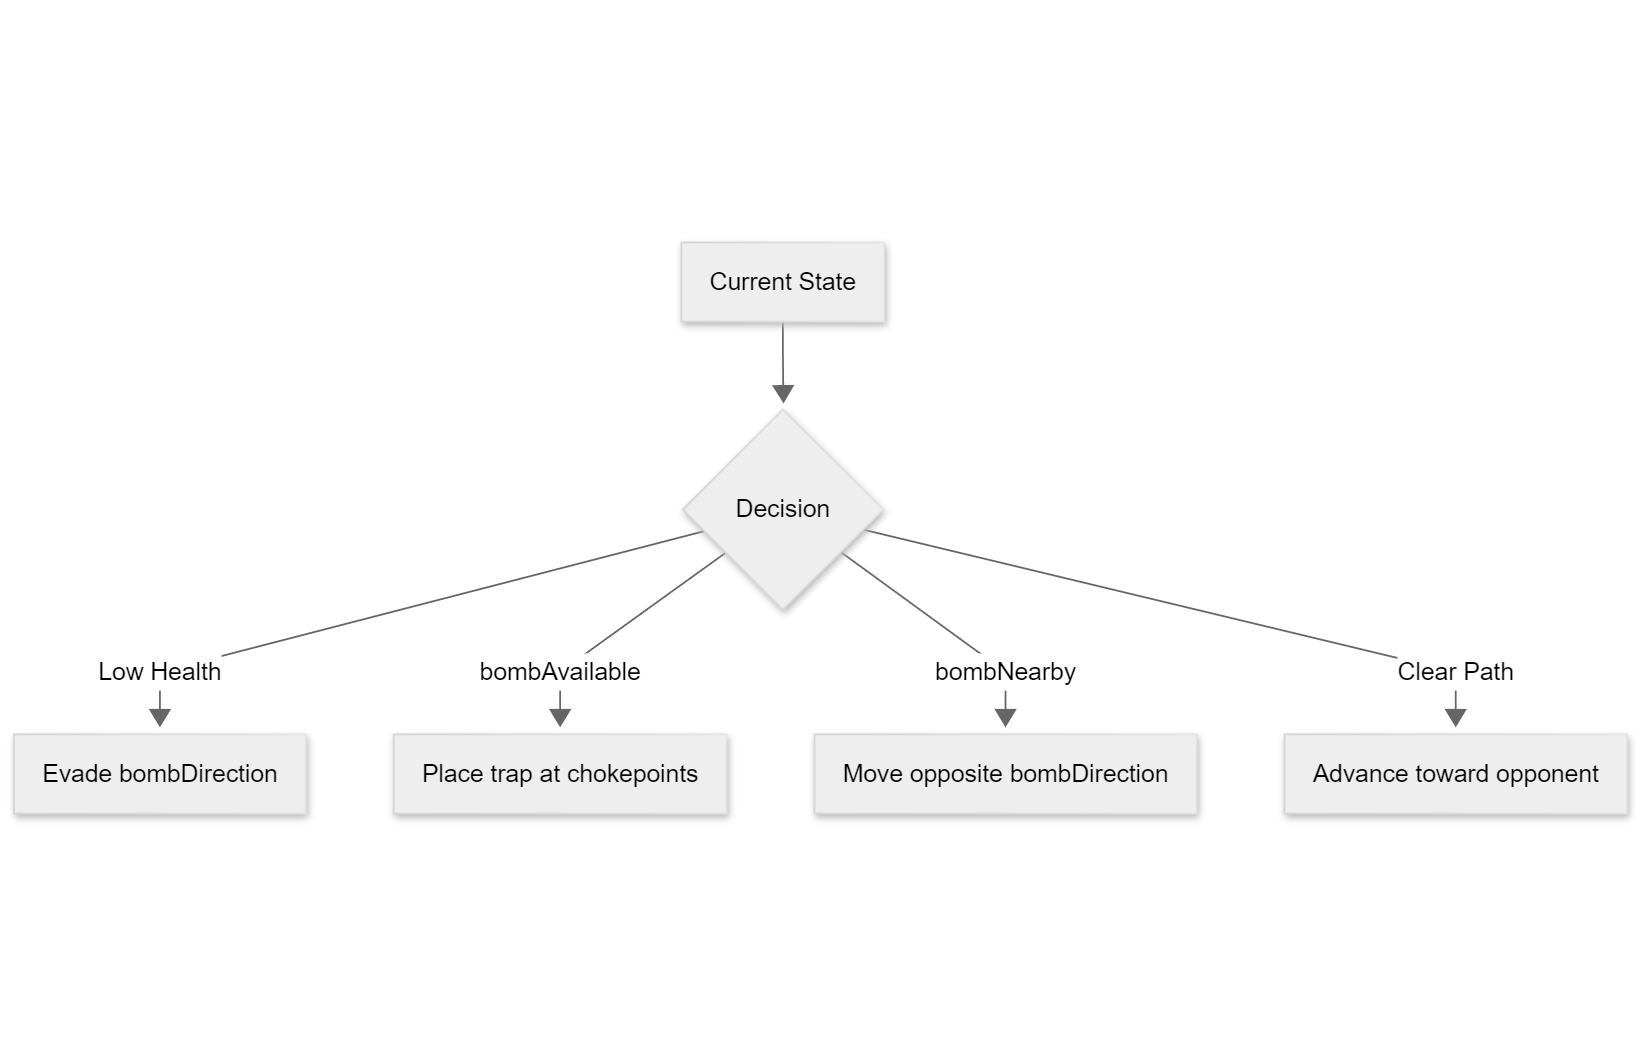
\includegraphics[width = 1\linewidth]{pictures/possibleActionsPlayer.png}
      \caption{\label{fig:possibleActionsPlayer}A diagram on the possible actions of a player}
      \end{figure}
Due to constrained optimization (e.g., state/action of the game), Genetic Algorithms are a perfect choice for this task \cite{popescu2025}: 
\textit{``Genetic Algorithms (GAs) were selected for their ability to handle complex combinatorial optimization problems [...] and to encode domain-specific constraints"} (Section 1).

The core steps of a typical genetic algorithm can be described as follows:
\begin{itemize}
    \item \textbf{Population Base}: Initialize a population from valid chromosomes, i.e. a set of strings that encodes any possible solution. Usually, the initial population is chosen randomly.
    \item \textbf{Evaluation}: Each population solution is evaluated on the basis of a predetermined fitness function.
    \item \textbf{Selection}: Reproductive opportunities are allocated to the chromosomes that represent a better solution to the target problem, and such solutions are selected to form a 'mating pool' for the next generation.
    \item \textbf{Crossover and Mutation}: The selected individuals are then combined to produce offspring by exchanging genetic material. Sometimes small changes can happen in the genetic material, such as bit flips. All of this ensures good exploration of the solution space and diversity.
    
\end{itemize}
These steps are repeated for a number of times until an ending criterion is reached.

\begin{figure}
\centering
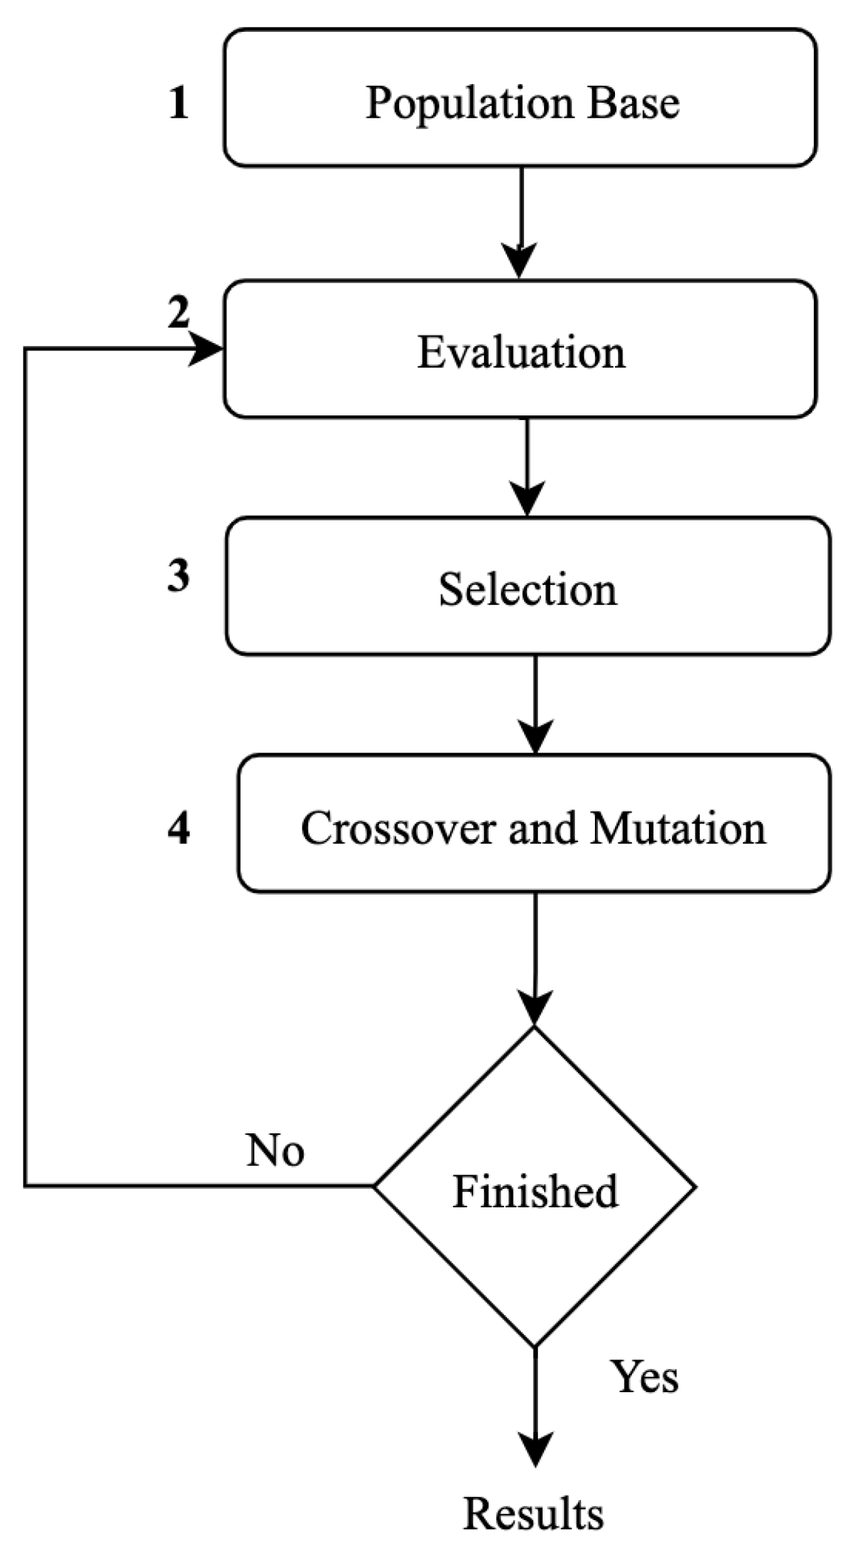
\includegraphics[width = 0.4\linewidth]{pictures/Steps-of-Genetic-Algorithms.png}
\caption{\label{fig:Steps-of-Genetic-Algorithm}A diagram on the steps of a genetic algorithm}
\end{figure}


\subsection{Robo Maze Blast's Default AI Agent}
The game has its own AI agents that will play against the player in the absence of in-real-life adversaries. They share a common behavior and reasoning that can be visualized with the finite-state machine, as shown in 
Figure 3.

%\begin{figure}
%
\includegraphics[width = 1\linewidth]{pictures/bomberman_finite_state_machine 1.png}
%\caption{\label{fig:bomberman_finite_state_machine 1}Finite-state machine of game's AI agent}
%\end{figure}



\section{Fine-tuning agent behaviors with jenetics}


\subsection{Differential Evolution}

\subsection{Agent Behavior}

\subsection{The Reward Metrics}
The fitness function determines which agent behaviors are rewarded, and which are penalized.
\begin{table}[htbp]
\centering

\caption{Agent Reward and Penalty Values}

\begin{tabular}{l|l}
\textbf{Action} & \textbf{Points}  \\
\hline
Movement & +1 (per step) \\
\hline
Place Bomb & +75 (per bomb) \\
\hline
Blow Wall & +150 (per wall) \\
\hline
Kills & +750 (per player) \\
\hline
Death  & -500  \\
\hline
Suicide & -500 \\
\hline
Win without kills & +200  \\
\hline
Win with kills & +1000  \\
\hline
\end{tabular}
\end{table}


\section{Evolutionary Training with Human Data and Jenetics}

\subsection{Approach Overview}
The planned approach uses human gameplay recordings to train AI agents through Jenetics' genetic algorithm framework. This creates a two-phase process:
\begin{enumerate}
	\item \textbf{Data Collection}: Record human player decisions as (state, action) pairs
	\item \textbf{Evolutionary Training}: Use recordings to seed initial GA populations, evolving agents that mimic human-like strategic patterns
\end{enumerate}

\subsection{Enhanced State Representation}
State vectors include proximity analysis of adjacent tiles:
\begin{verbatim}
	state = [
	normX, normY,           // Player position (normalized)
	bombAvail,              // 1 if bomb available, else 0
	bombNear,               // 1 if bomb in blast radius, else 0
	{up, down, left, right} // Adjacent tile analysis:
	// -1: Enemy present | 0: Empty | 1: Destructible | 2: Wall
	]
\end{verbatim}

\textit{Example}: \texttt{[0.35, 0.60, 1, 1, -1, 0, 2, 1]} indicates:
\begin{itemize}
	\item Player at (35\% X, 60\% Y)
	\item Bomb available \& nearby
	\item Enemy above | Empty below | Wall left | Destructible right
\end{itemize}

\subsection{Elo System Integration}
We propose implementing an Elo-based evaluation framework:
\begin{equation}
	\Delta Elo = K \times (S_{actual} - S_{expected})
\end{equation}
where 
\begin{equation}
	S_{expected} = \frac{1}{1 + 10^{(Elo_B - Elo_A)/400}}
\end{equation}

This would enable:
\begin{itemize}
	\item Dynamic agent ranking through automated tournaments
	\item Quantitative measurement of strategy improvements
	\item Fitness evaluation via Elo changes rather than fixed point systems
\end{itemize}

\subsubsection{Data Collection Protocol}
We planned 5 hours of gameplay recording across 3 skill levels:
\begin{itemize}
	\item \textbf{Novice (1 hrs):} Focus on survival patterns
	\item \textbf{Intermediate (3 hrs):} Balanced playstyle
	\item \textbf{Expert (1 hrs):} Advanced bombing strategies
\end{itemize}
Raw data would undergo preprocessing to remove:
\begin{enumerate}
	\item Idle movements (consecutive \texttt{STAY} actions)
	\item Input errors (rapid direction changes)
\end{enumerate}

\subsubsection{Elo Implementation Details}
The $K$-factor would be dynamically adjusted:
\begin{equation}
	K = \begin{cases} 
		32 & \text{for } Elo < 1600 \\
		24 & \text{for } 1600 \leq Elo < 2000 \\
		16 & \text{otherwise}
	\end{cases}
\end{equation}
Tournaments would follow Swiss-system pairing with:
\begin{itemize}
	\item 10 rounds per generation
	\item 3-minute time control
	\item Mirror matchups to eliminate map bias
\end{itemize}

\subsection{Revised Jenetics Workflow}
\begin{algorithm}[t]
	\caption{Data-Driven Evolutionary Training}
	\label{alg:jenetics_workflow}
	\DontPrintSemicolon
	\SetKwFunction{Eval}{EvaluateFitness}
	\SetKwFunction{Select}{TournamentSelection}
	\SetKwFunction{Crossover}{SinglePointCrossover}
	\SetKwFunction{Mutate}{GaussianMutate}
	
	\textbf{Input:} Recorded gameplay dataset $D$\;
	\nl\textbf{Initialization:} 
	population $\leftarrow$ sampleChromosomes($D$)\;
	generation $\leftarrow$ 0\;
	
	\BlankLine
	\nl\textbf{Evolution Loop:}\;
	\nl \While{not converged}{
		\Eval{population} \tcp*{Using EloChange metric}\;
		parents $\leftarrow$ \Select{population, size=5}\;
		offspring $\leftarrow$ \Crossover{parents, rate=0.8}\;
		population $\leftarrow$ \Mutate{offspring, rate=0.15}\;
		updateEloRatings(population)\;
		\If{generation \% 10 == 0}{
			pruneWorst(population, 0.2)\tcp*{Remove bottom 20\%}
		}
		generation $\leftarrow$ generation + 1\;
	}
	
	\nl\textbf{Output:} 
	bestAgent $\leftarrow$ getHighestElo(population)\;
\end{algorithm}

\subsubsection{Parameter Selection}
Rates were determined via grid search:
\begin{table}[h]
	\centering
	\begin{tabular}{c|c|c}
		Mutation & Crossover & Win Rate \\ \hline
		0.10 & 0.75 & 58\% \\
		0.15 & 0.80 & 63\% \\
		0.20 & 0.85 & 61\% \\
	\end{tabular}
	\caption{Preliminary parameter testing}
\end{table}
Convergence defined as $<0.5\%$ Elo change over 15 generations.


\subsection{Addressing Implementation Challenges}
While time constraints prevented full execution, the framework resolves key integration issues:
\begin{itemize}
	\item \textbf{State representation} now handles complex game conditions
	\item \textbf{Automated Elo tracking} replaces manual agent comparison
	\item \textbf{Data-driven initialization} avoids random starting points
\end{itemize}

\begin{figure}
	\centering
	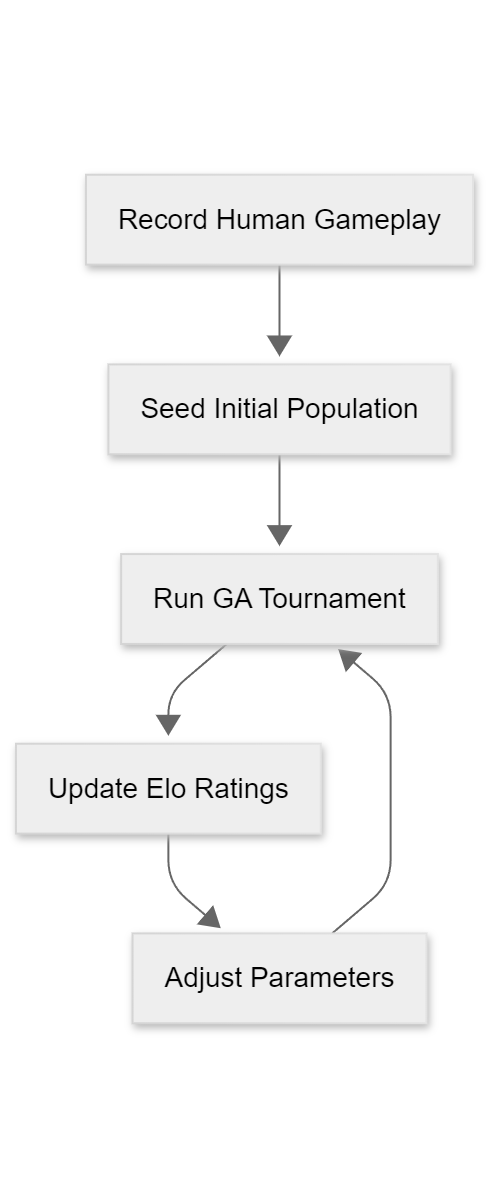
\includegraphics[width=0.7\linewidth]{pictures/workflow}
	\caption[Critical path for future work]{}
	\label{fig:workflow}
\end{figure}

\section{Tree-Based Genetic Programming}
\subsection{Introduction}

The evolutionary algorithm chosen for the second implementation is tree-based genetic programming (GP). This approach offers multiple benefits: 
First, it is highly flexible. The tree structure allows a wide range of programs to be represented by the algorithm. 
Furthermore, GP can "discover novel and unexpected solutions that may not be apparent to human programmers," as the algorithm is not biased toward favoring certain approaches over others, as long as they are within the rules set by the programmer or hardware. 
Additionally, GP can easily adapt to changing requirements and inputs, making it highly adaptable. 
This approach was chosen due to its high flexibility. While the initial training phase against the already implemented AI players might be more challenging due to the complexity of the setup compared to other algorithms like Differential Evolution or regular Genetic Algorithms, the benefits of flexibility and adaptability to new circumstances are promising in an environment where multiple evolutionary algorithms compete against each other. 

\subsection{Design Decisions}

The implementation of the algorithm is encapsulated in the GeneticPlayer class. This class does not inherit from the AIPlayer class, which already contains significant functionality. Inheritance was avoided because the setup of genetic programming differs significantly from "regular" genetic algorithms. GP uses a tree structure and consists of multiple components (functions, terminals, and constants). Terminals represent the leaf nodes of the tree, whereas functions branch out, increasing the complexity of the tree.The GeneticPlayer class contains an abstract static class called Operation, which serves as the base for all terminals and functions. The respective terminals and functions inherit from Operation. The terminals include basic movement operators such as MoveUp, MoveDown, MoveLeft, MoveRight, and Stay, which represent movements in the game along the x- and y-axes. Additional terminals include IsTargetZone, CheckForBomb, PlaceBomb, CheckForExtra, GetDistanceToEnemy, and three constant values. These terminals encapsulate functionality already implemented for the AIPlayer, allowing the GP to iterate over it. The constant values are arbitrary defaults that can be adjusted based on the algorithm's performance or goals.The algorithm also relies on two operations: GreaterThan and IfElse. GreaterThan has an arity of 2, meaning it compares two values, returning 1 if the first value is greater than the second and 0 otherwise. IfElse has an arity of 3. It checks whether the first value is greater than 0. If true, it forwards the value t[1]; otherwise, it forwards t[2].The core of the GP is the initializeGP method. In this method, functions and terminals are initialized, and the maximum tree depth is set. During the training phase, a depth of 5 was used, but this can be adjusted based on performance. The engine combines the algorithm's constraints with the fitness function. Parameters such as population size, mutation rate, and crossover rate can be manually adjusted depending on the algorithm's performance. The result performs the actual training by streaming the data and applying the constraint of the number of generations. Finally, the best strategy is returned.The fitness function is where the actual training occurs. Each time the fitness function is called, a new game and playground are initialized. A new GeneticPlayer and three new AIPlayer instances are created. Notably, during the training phase, a specific method, addAIForFitness, was implemented in the Game class. This method does not start the threads typically used during a game simulation. The operations and terminals are linked to the newly created GeneticPlayer. 
\begin{alltt}
	for (int i = 0; i < 1000; i++) \{
	if (!game.isRunning() || goodboy.isDead()) \{
	System.err.println("Fitness: Stopped at iteration " + i + 
	", game running = " + game.isRunning() + 
	", GoodBoy dead = " + goodboy.isDead());
	steps = i;
	break;
	\}
	for (Player player : game.getPlayers()) \{
	if (player instanceof AIPlayer aip) \{
	System.err.println("Fitness: AIPlayer " + 
	aip.getNickname() + " tick");
	aip.tick();
	\} else \{
	GeneticPlayer gp = (GeneticPlayer) player;
	double result = gp.program.eval();
	System.err.println("Fitness: GeneticPlayer tick, " +
	"result = " + result + ", position = (" + 
	gp.gridX + "," + gp.gridY + ")");
	if (result >= 1.0 && result <= 4.0) \{
	successfulMoves++;
	\}
	\}
	\}
	game.tick();
	\}
\end{alltt}

In the loop, the player performs a maximum of 1,000 iterations before being forced to terminate. The loop is interrupted if the player dies or the game is no longer running, simulating a real environment where the GP interacts with AIPlayer instances. In each iteration, both the AIPlayer and GeneticPlayer call their tickmethods, selecting a new action and synchronizing their current state. After all players have synchronized, the game synchronizes with game.tick. During game.tick, selected bombs detonate, extras collected by players in the previous period modify their bomb range or capacity, and players may be killed by exploding bombs and removed from the game. Successful moves by the GP are recorded during the loop, as they impact the overall fitness.The fitness function consists of multiple components: 
\begin{itemize}
      \item survivalTime 
      \item extrasCollected 
      \item deathPenalty 
      \item moveReward 
\end{itemize}
Since the algorithm aims to minimize the fitness function, beneficial actions for the GP receive a negative multiplier, while harmful actions receive a positive multiplier. Notably, the fitness function currently ignores the number of opponents the GP kills, meaning aggressive behavior does not affect fitness. This design choice promotes defensive behavior, prioritizing survival over aggression. The goal is for the player to survive as long as possible, leading to longer games compared to aggressive strategies where the player either dies or kills quickly. This defensive approach, inspired by strategic games like chess where top players prioritize avoiding mistakes over attacking, is reinforced by a high deathPenalty and a strong emphasis on survivalTime as a negative metric.The GeneticPlayer class also includes a tick method, called by the GeneticPlayerThread, which is started in a real game environment to visually observe the player's behavior. 

\subsection{Issues}
The algorithm in its current form does not perform as intended. Several issues arose during implementation, some of which remain unresolved: 
\begin{enumerate}
      \item Not inheriting from the AIPlayer class. 
      The primary issue, likely causing subsequent problems, was the decision not to inherit from the AIPlayerclass. Although this was a deliberate choice initially, it likely caused more harm than good. Much of the functionality was copied with slight adjustments, adding redundant code without significant value. The GeneticPlayer inherits from the Player class, sharing many variables with AIPlayer. This required moving some code, such as the die and isDead methods, from AIPlayer to Player to make it accessible to the GP.
      \item Adjusting classes that were already functional. 
      Other classes, such as the Game class, were modified to include the tick method, which synchronizes player actions within a time frame. However, these adjustments introduced additional issues, complicating debugging.cDuring the project, console output showed that the player performed actions like moving up and down, which sometimes succeeded and sometimes failed depending on obstacles like walls. However, the player never placed bombs. Debug print statements revealed that the condition player.bombs.size() < player.bombCount was never true, indicating that bombs always contained a bomb before the output statement was triggered. This led to replacing many System.out.println() statements with System.err.println(), suspecting that threading issues were affecting the print statements (as threads were initially started for all AIPlayer instances). This hypothesis was confirmed, revealing another issue: the players and bombs were not synchronized.
      \item Synchronization of player behavior. 
      While AIPlayer instances were bound to a tick every 300 ms, bombs exploded every 4,000 ms. The GP, however, was not constrained by these timings, operating only limited by CPU capacity. This caused the GP to perform significantly more iterations before a bomb exploded, leading to poor assumptions about its behavior after placing a bomb, often resulting in the player committing suicide. Ultimately, AIPlayer threads were disabled to remove artificial constraints designed for a realistic gaming experience, allowing the simulation to run without being bound by these limitations. The above issues have left the algorithm only partially functional. Synchronization of triggered behaviors (bomb explosions, AIPlayer actions, and GeneticPlayer actions) caused significant problems. Many issues could have likely been avoided by inheriting most behavior from AIPlayer. The synchronization problem could have been mitigated by aligning the GP's tick time with that of the AIPlayer. However, this would have slowed the algorithm or reduced its quality, as the complexity and population size would need to be significantly reduced to maintain performance. 
\end{enumerate}
\bibliographystyle{alpha}
\bibliography{sample}

\end{document}
